Onto Wednesday! Today starts with a keynote by Ian Goodfellow. \\

\subsection{Invited Talk: Ian Goodfellow on Adversarial Learning}

Topic: Adversarial ML! And how it relates to other topics. \\

Traditional ML: based on optimization -- choose a cost function $J(\theta_1,\theta_2)$, find $\theta_1$ and $\theta_2$ that minimize $J$. This works great for classifiers! We can gradually minimize $J$ through various techniques until we find the right parameters. \\

But: lots of other parameters we can't really optimize. \\

$\ra$ Let's instead fall back to game theory. Two players play a game -- player 1 wants to minimize the score of the game, player 2 wants to maximize. If it converges, we find an equilibrium point.\\

\begin{figure}
    \centering
    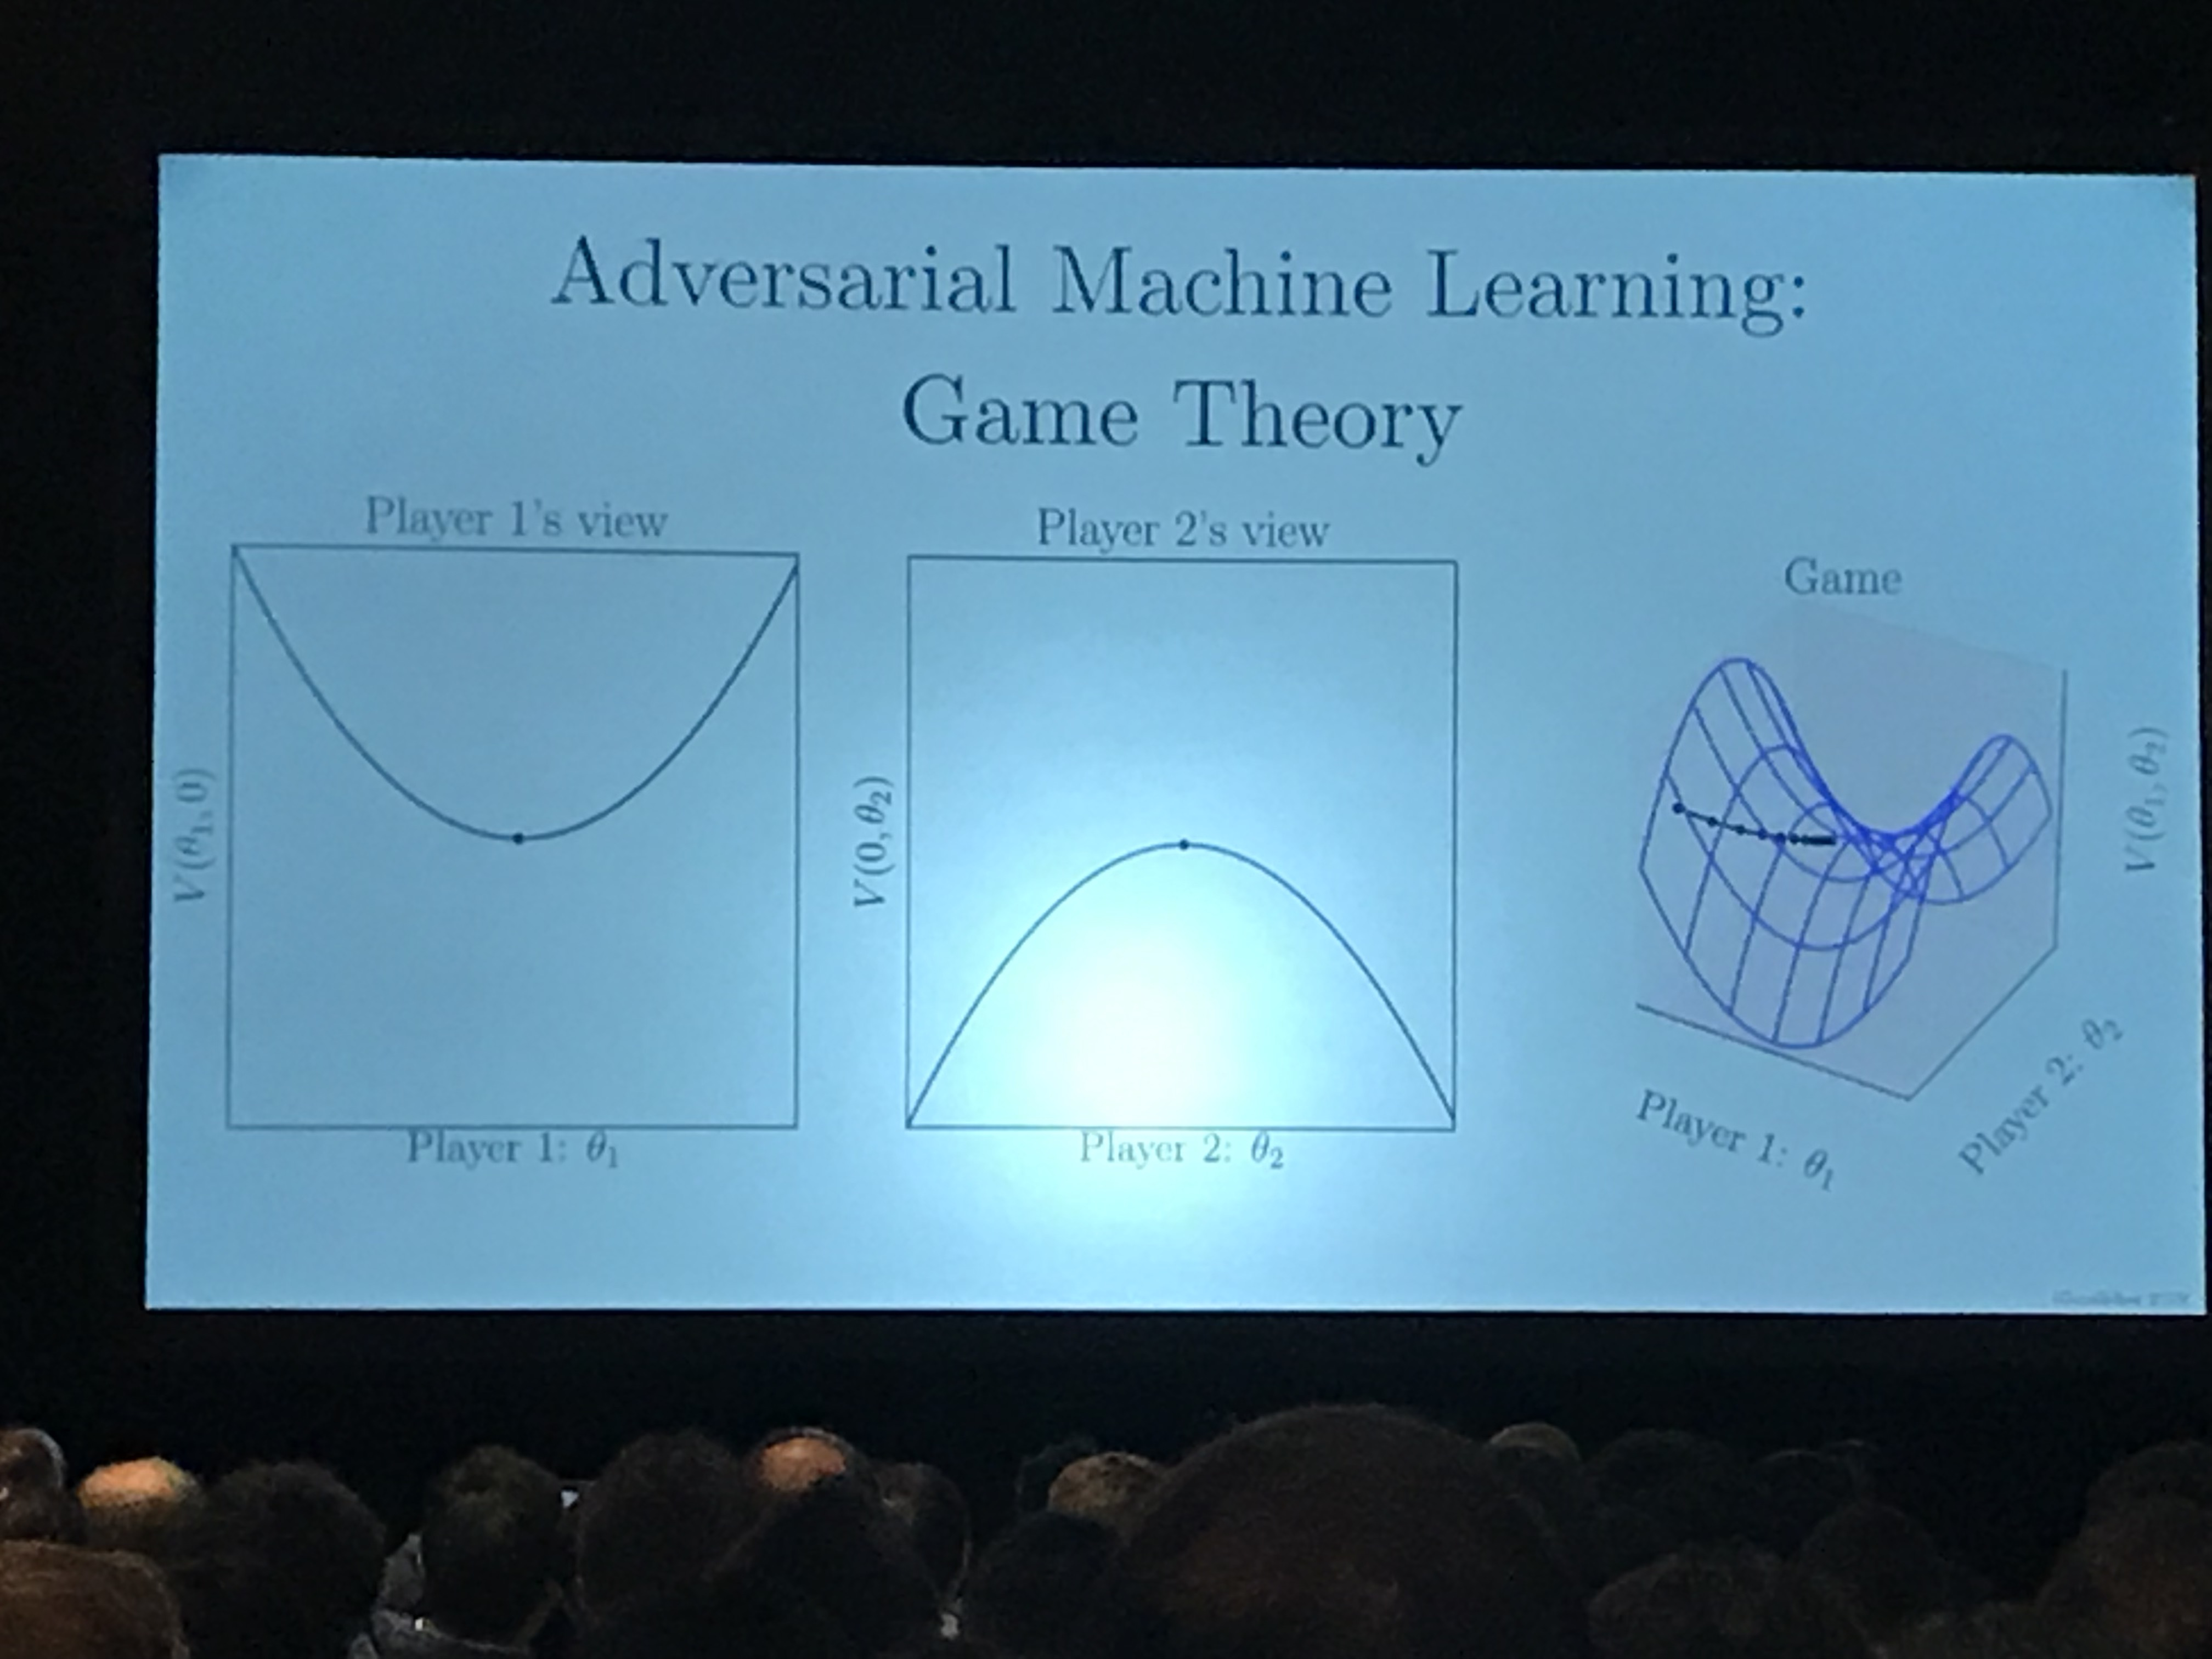
\includegraphics[width=0.5\textwidth]{images/game.JPG}
    \caption{Game theory and optimization.}
    \label{fig:games}
\end{figure}

Cambrian explosion of ML research topics:
\begin{itemize}
    \item used to be (2007), let's get ML to work! 
    
    $\ra$ Then, one that works, we can do vision/NLP and so on.
    
    \item Now, with ML working, we can go on to do loads of other things (neuroscience, security, RL, domain adaption, and so on).
    
    $\ra$ So we're starting to see that happen.
\end{itemize} 

\subsubsection{Generative Modeling}

Main idea: take a collection of training data, and learn a distribution that can generate similar samples~\cite{karras2017progressive}. \\

Use Generative Adversarial Nets (GANs)~\cite{goodfellow2014generative}:
\begin{itemize}
    \item Train a 1) generator to generate images, starting out random
    \item Train a 2) discriminator, to recognize fake images from real images.
    \item These two play a game to convergence.
\end{itemize}

\begin{figure}[h!]
    \centering
    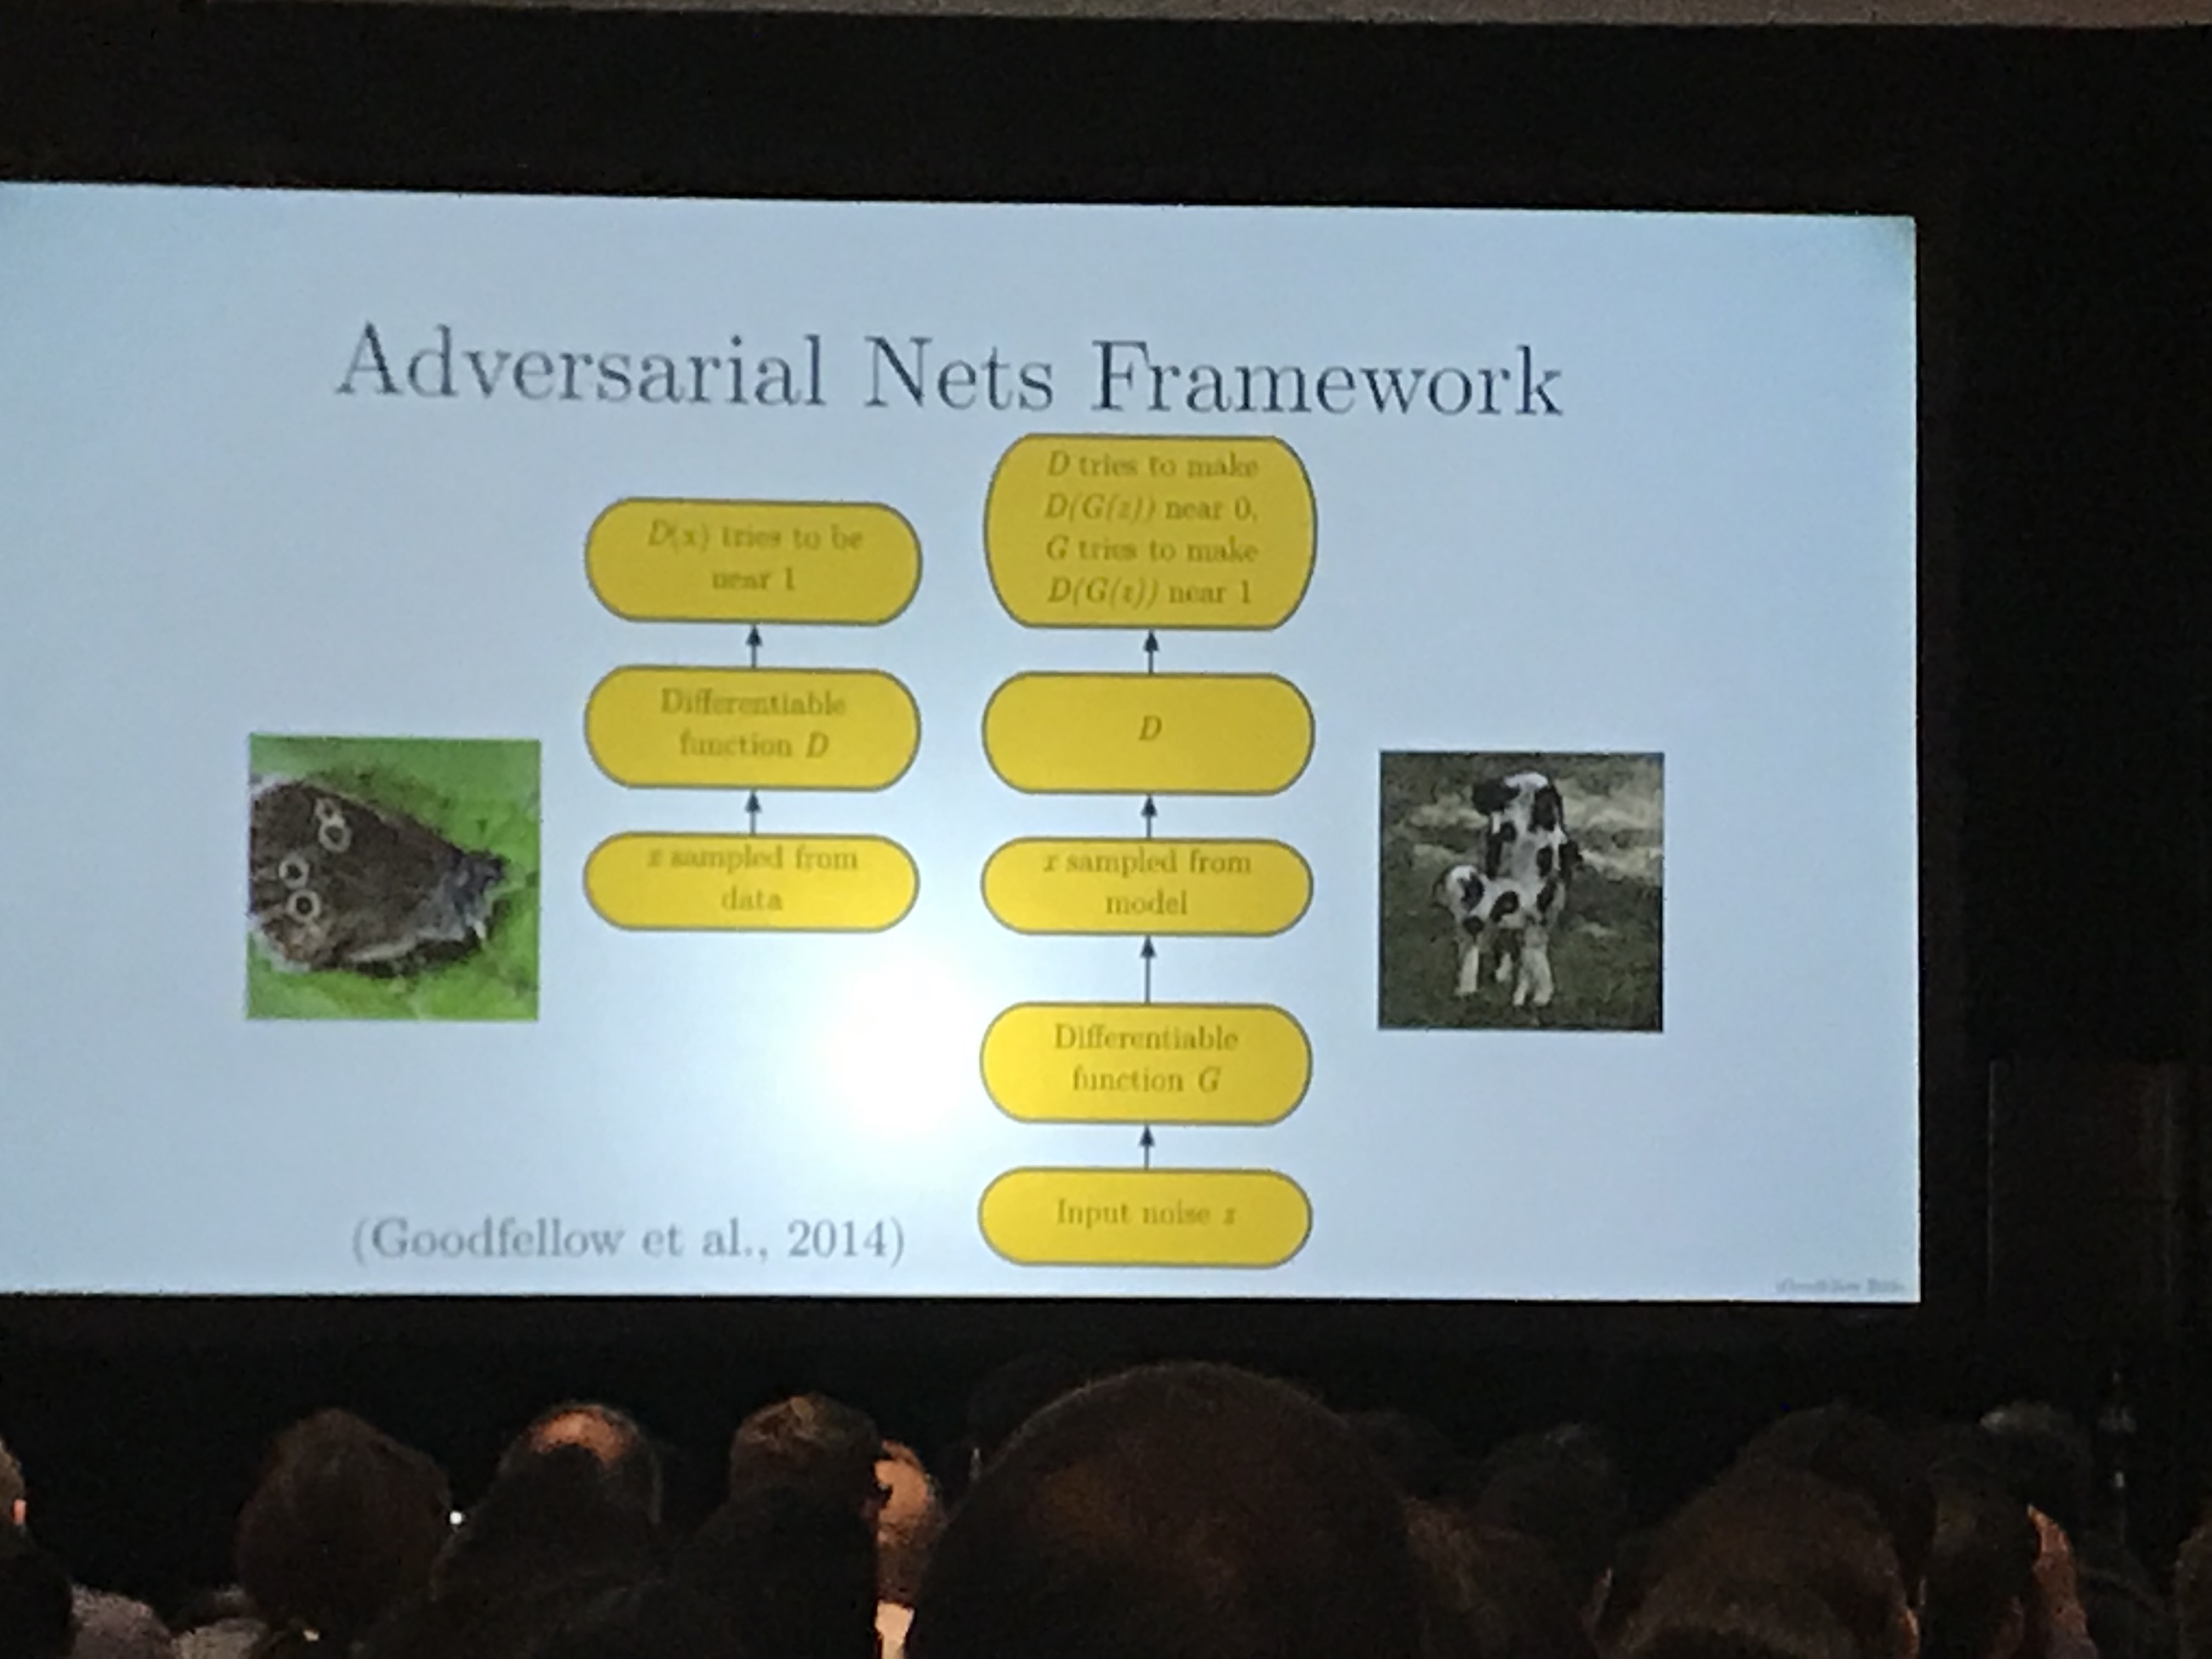
\includegraphics[width=0.5\textwidth]{images/gans.JPG}
    \caption{GAN Framework.}
    \label{fig:gan}
\end{figure}

Rapid progress in image generation (and especially faces -- see Figure~\ref{fig:gan_prog}). Also progress in imagenet, but it's harder because so many more classes. \\


\begin{figure}[h!]
    \centering
    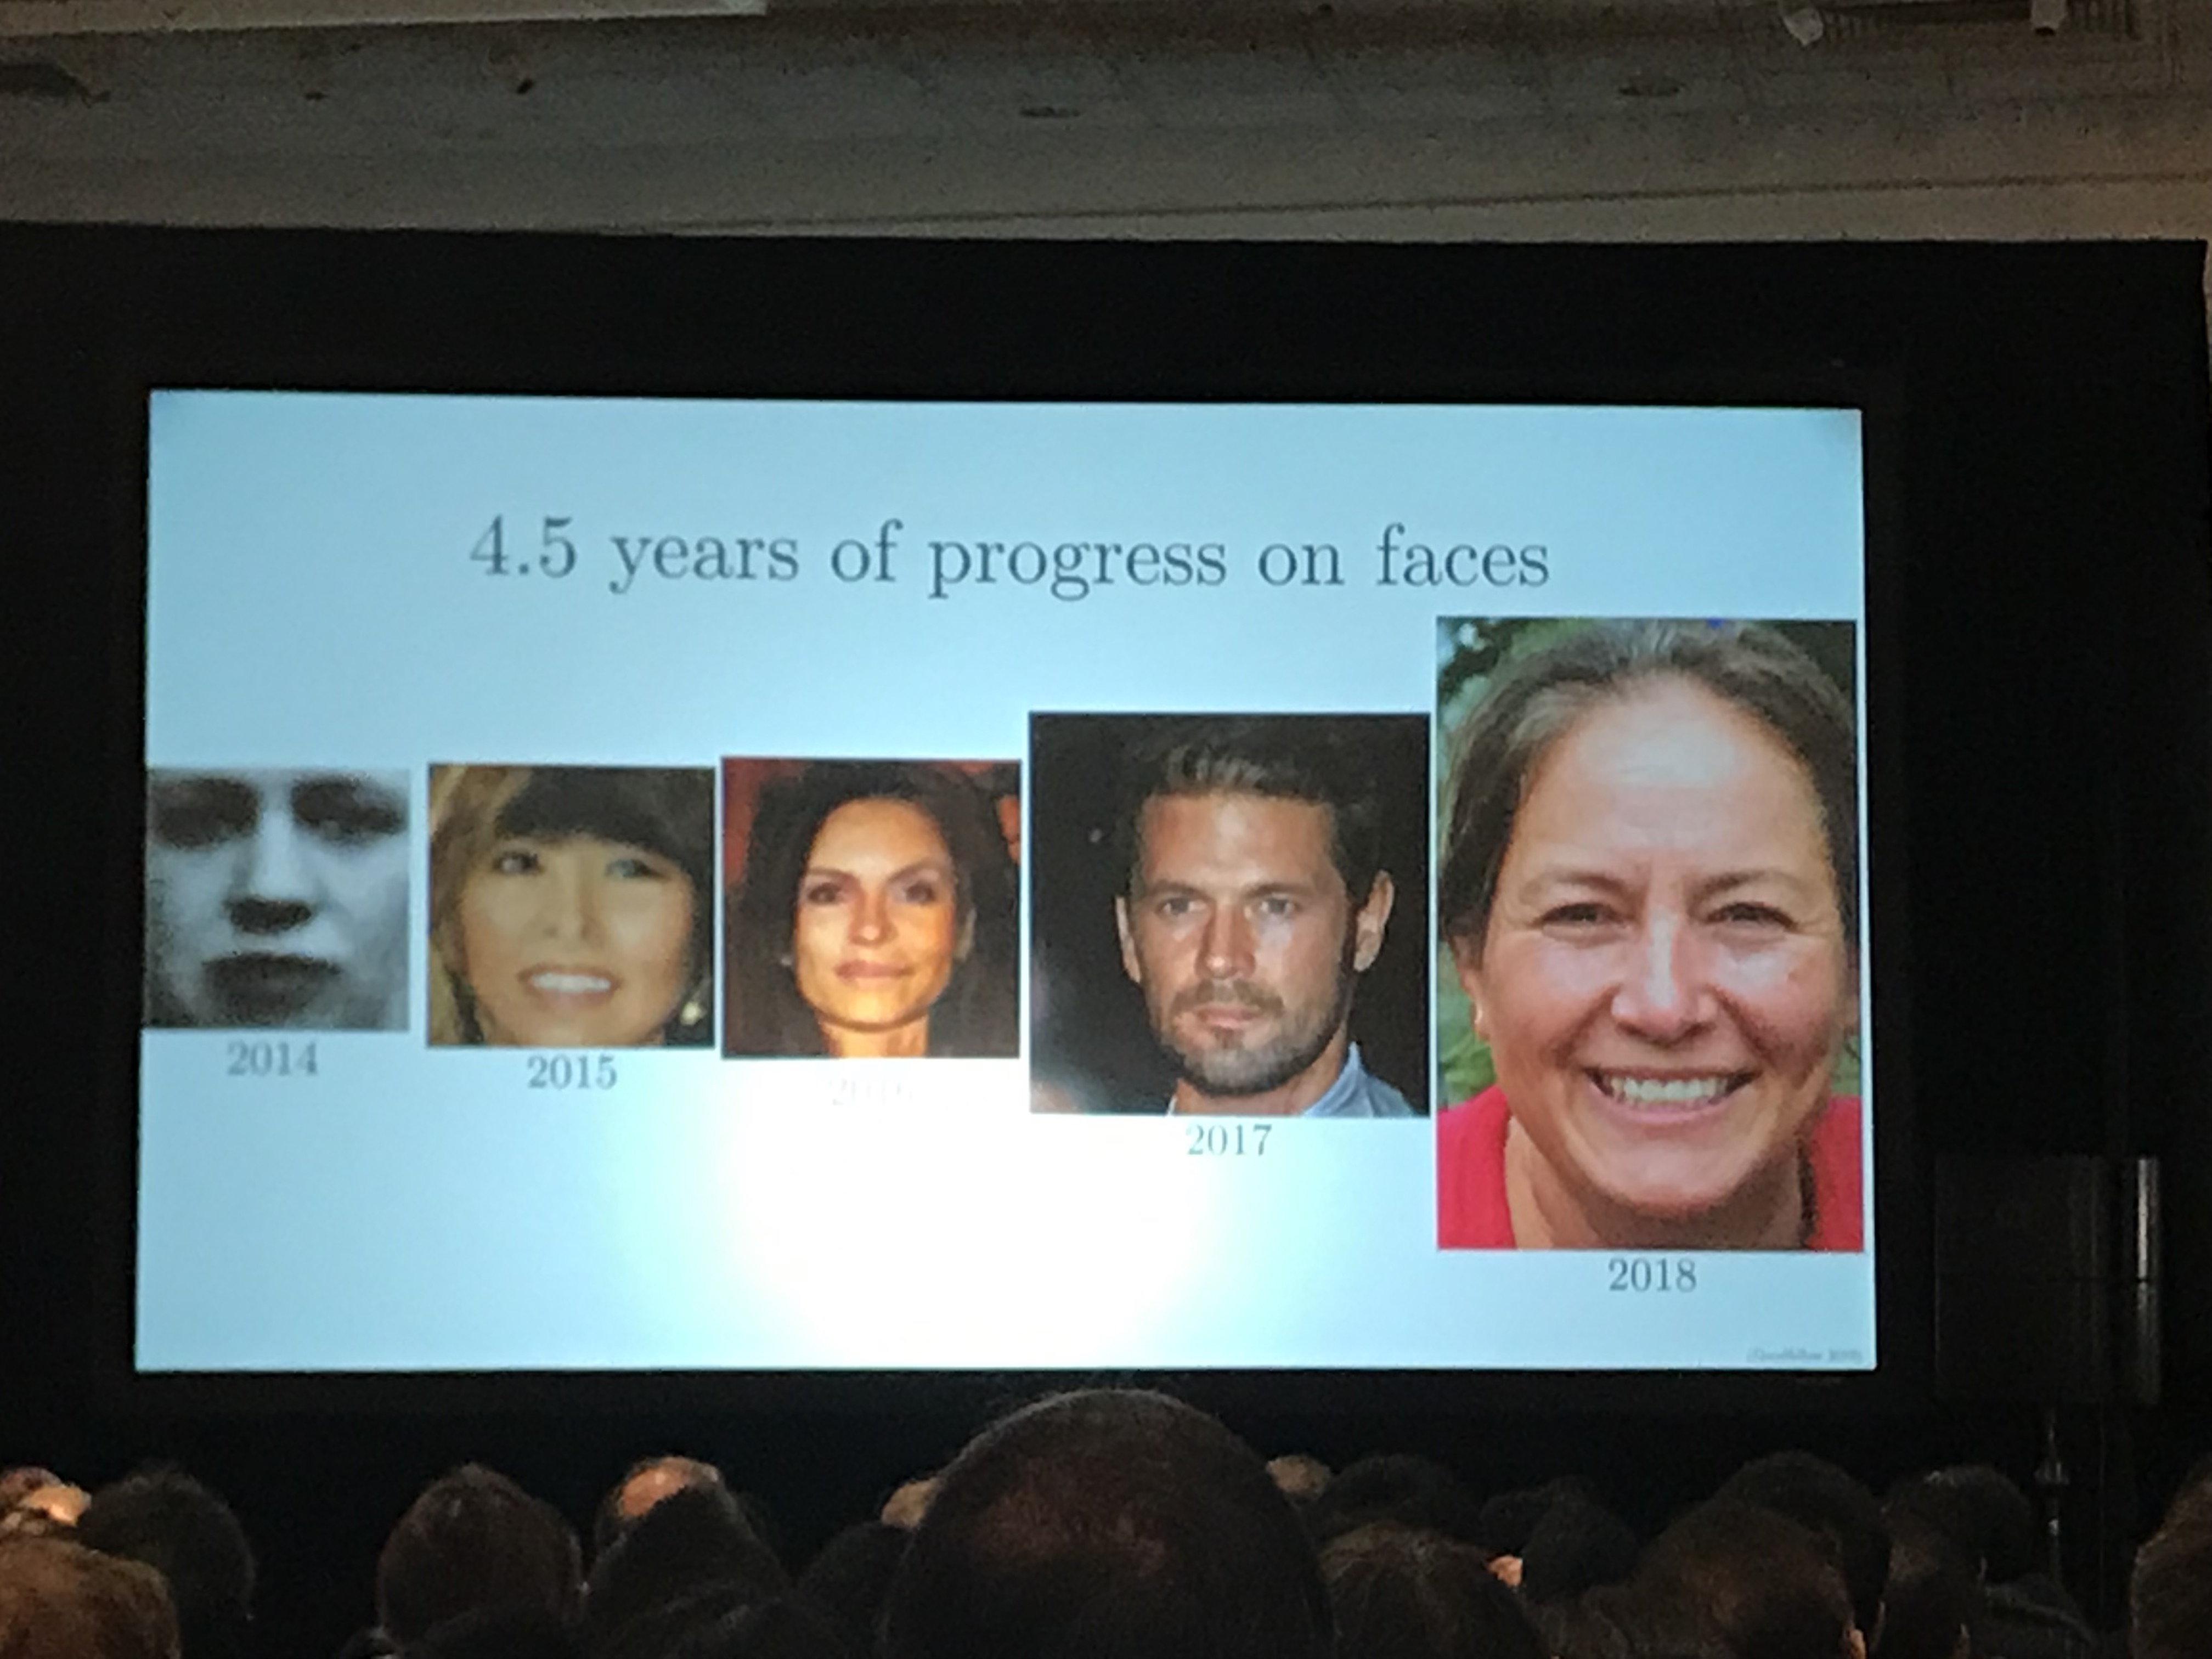
\includegraphics[width=0.5\textwidth]{images/gan_progress.JPG}
    \caption{GAN Progress.}
    \label{fig:gan_prog}
\end{figure}


GANs solve the generative modeling problem, but also the domain translation problem -- can translate video stream during the day to video streams at night {\it without paired day-night examples}. \\

Cool example: cycleGan~\cite{zhu2017unpaired} converts horses to zebras. Also lets us diagnose some issues with the techniques -- CycleGAN only does image-to-image, so it's not targeting video coherence. Also picks up on 


\begin{figure}[h!]
    \centering
    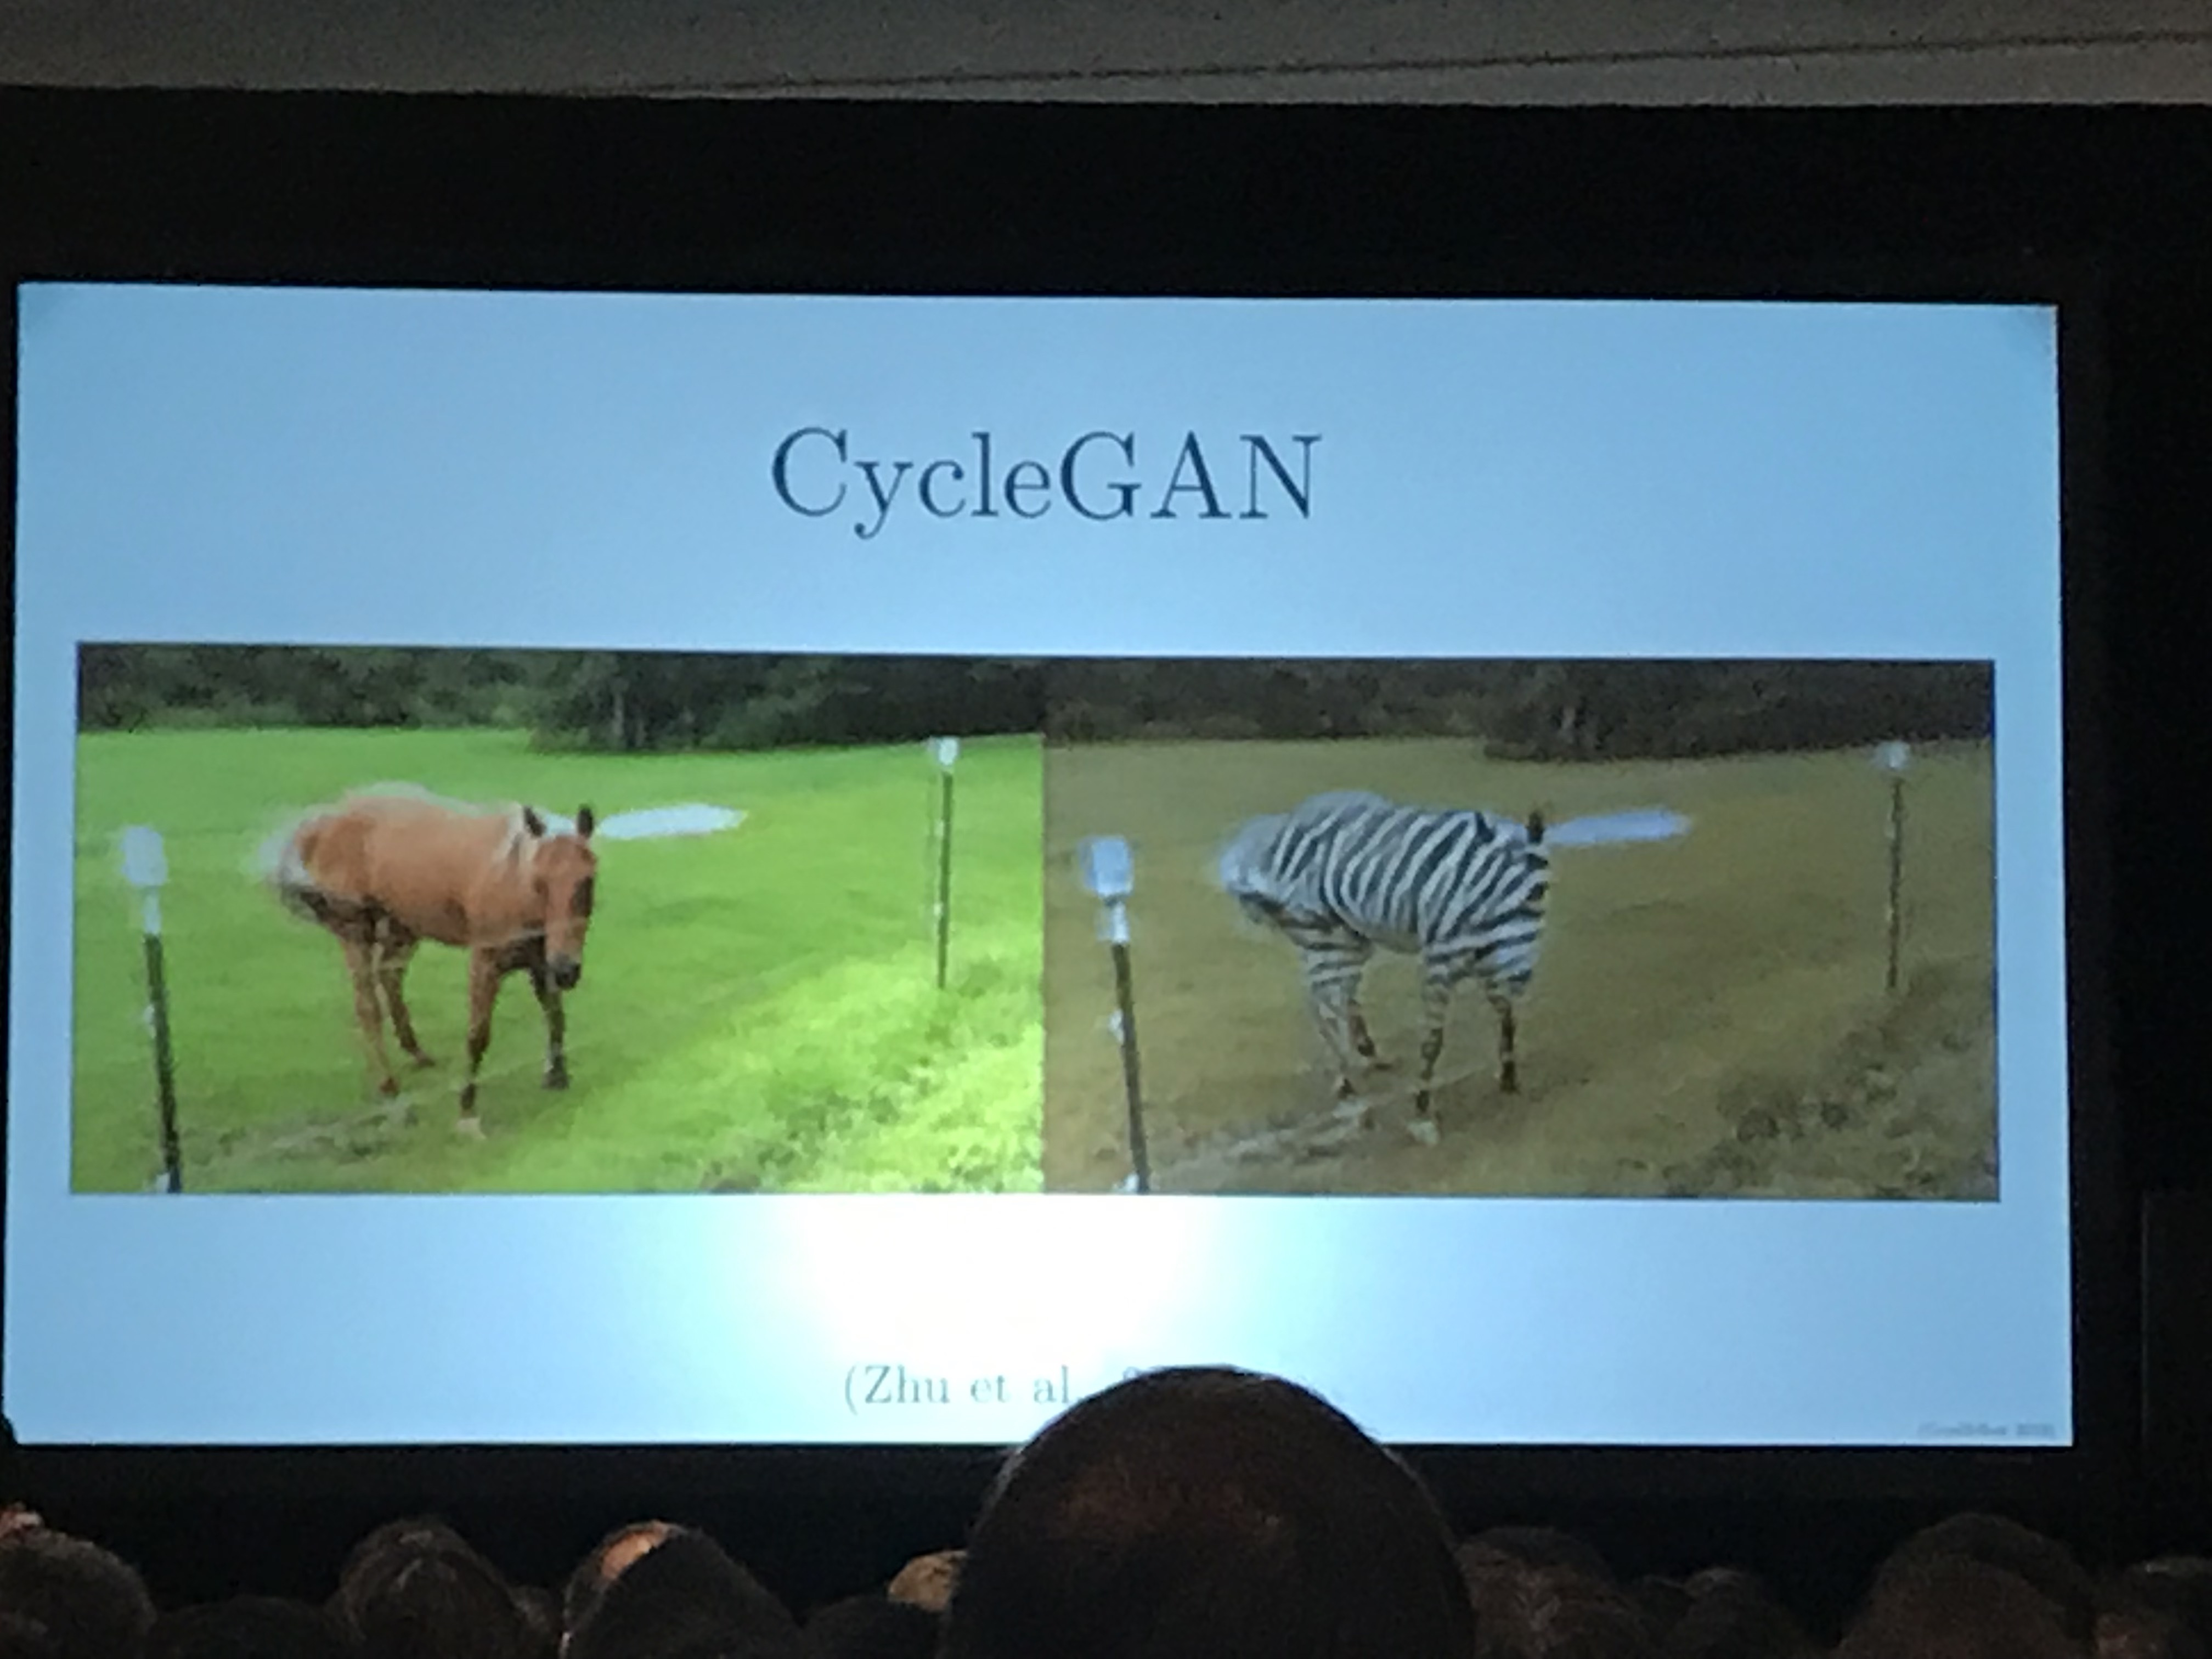
\includegraphics[width=0.5\textwidth]{images/zebra.JPG}
    \caption{CycleGAN turns horses into zebras (actually a video).}
    \label{fig:zebra}
\end{figure}

Also showed an {\it amazing} video of a fake/animated dancer that can be used to change video stream of people to dance in that style. \\

{\bf Application:} New company that generates custom made dental crowns very quickly, which dramatically improves over the traditional method for making crowns. \\

{\bf Prediction:} Fashion! Should be possible to generate clothing that fits well/satisfies individual tastes. \\

\subsubsection{Recent Developments}

Basically: ML works now! So we can do all sorts of cool things, including:
\begin{itemize}
    \item Security
    \item Model-Based Optimization
    \item Reinforcement learning
    \item Fairness and accountability
    \item Neuroscience
\end{itemize}


First, some new ideas in GANs:
\begin{itemize}
    \item Self-Attention~\cite{wang2018non}: Attention mechanism you can add to a CNN that lets you focus on other parts of previous layers' feature maps, given a piece that the network just generated~\cite{} -- so, when it generates an eye of an animal, you can highlight the eye and see what it was focused on.
    
    $\ra$ Not constrained to any shape of attention region -- it can highlight an arbitrary region.

    \item Also: BigGAN~\cite{brock2018large}, large scale TPU implementation. Can generate images at high resolution that are good enough to fool human observers.
\end{itemize}


{\bf Security:} \\

Adversarial Examples! We think these are the result of assuming i.i.d. data -- attackers can violate both ``i" assumptions. \\

$\ra$ attacker can choose examples not drawn from the same distribution (stop sign with graffiti, putting an apple in a mesh bag).
$\ra$ attacker can violate independence, too, to fool a model. \\

These completely work in the physical world too. \\

Advervarsarial training as a minimax problem:
\[
\theta^* = \argmin_\theta \bE_{x,y} \max_\eta[J(x,y,\theta) + J(x+y,\eta, \theta)]
\]

Open research direction: change the i.i.d. assumption and train on adversarial examples, too. Can often make classifiers more robust to these examples. \\

{\bf Model-Based Optimization:}

Idea: train an ML model, and instead of training it to label new data, we use it to train the search for new data points. \\

$\ra$ DNA Sequence design. \\

{\bf Reinforcement Learning:} \\

Recent work identifies adversarial examples for RL, too! \\

But, we can also use GANs to help RL. Consider Arthur Samuel's 1959 checkers player -- used self play to improve itself~\cite{brock2018large}, which is very much in use now. \\

GANs can be used to provide learned reward functions, as in SPIRAL~\cite{ganin2018synthesizing}. Can generate reward functions in the appropriate input domain (robot camera percepts). Usual MSE won't work, but GANs can actually provide a useful distance measure such that a robot can learn to solve robot problems. \\

{\bf Extreme Reliability:} We want extreme reliability for medical diagnosis, surgery robots, and other safety critical domains. \\

$\ra$ Adversarial machine learning might be able to produce extremely reliable systems because they are explicitly trained to be robust to attacks. \\

Virtual Adversarial Training~\cite{miyato2018virtual}: take an unlabeled example, but we know that it ought to be labeled the same whether or not an adversary messes around with it. Works {\it extremely} well for semi-supervised learning (sample efficient, regularizes well). \\

{\bf Domain Adaptation:} We train in one domain (perhaps where data is abundant) and test in another domiain. \\

$\ra$ A ``domain" here is a particular choice of distribtion for training -- ImageNet, videos of people walking down a street, and so on. \\

$\ra$ If we can achieve domain adaptation, pretty good evidence for reliable/robust generalization. \\

One main approach: Domain adaptation networks~\cite{ganin2016domain}. Idea: try to recognize the domain itself, which forces the discriminator to generalize well. \\

Another important instance of domain adaptation focuses on transferring from {\it simulated} training data to {\it real} data. Works well with recognizing where eyes are looking, for instance. \\

$\ra$ Can do robot grasping by training simulation and then actually grasp in the real world.\\

{\bf Fairness, Accountability, Transparency:} GANs can learn more fair representations \\

$\ra$ Fairness: An adversary tries to infer a sensitive variable $S$ from a representation. Learner tries to learn while making $S$ impossible to recover~\cite{edwards2015censoring}. \\

$\ra$ Transparency: Interpretability and adversarial learning should talk more. Interpretability means getting the right answer, while adversarial training means the learner is getting the ``right" thing. \\

{\bf Neuroscience:} \\

Adversarial examples affect both computer and time-limited human vision:

\begin{figure}
    \centering
    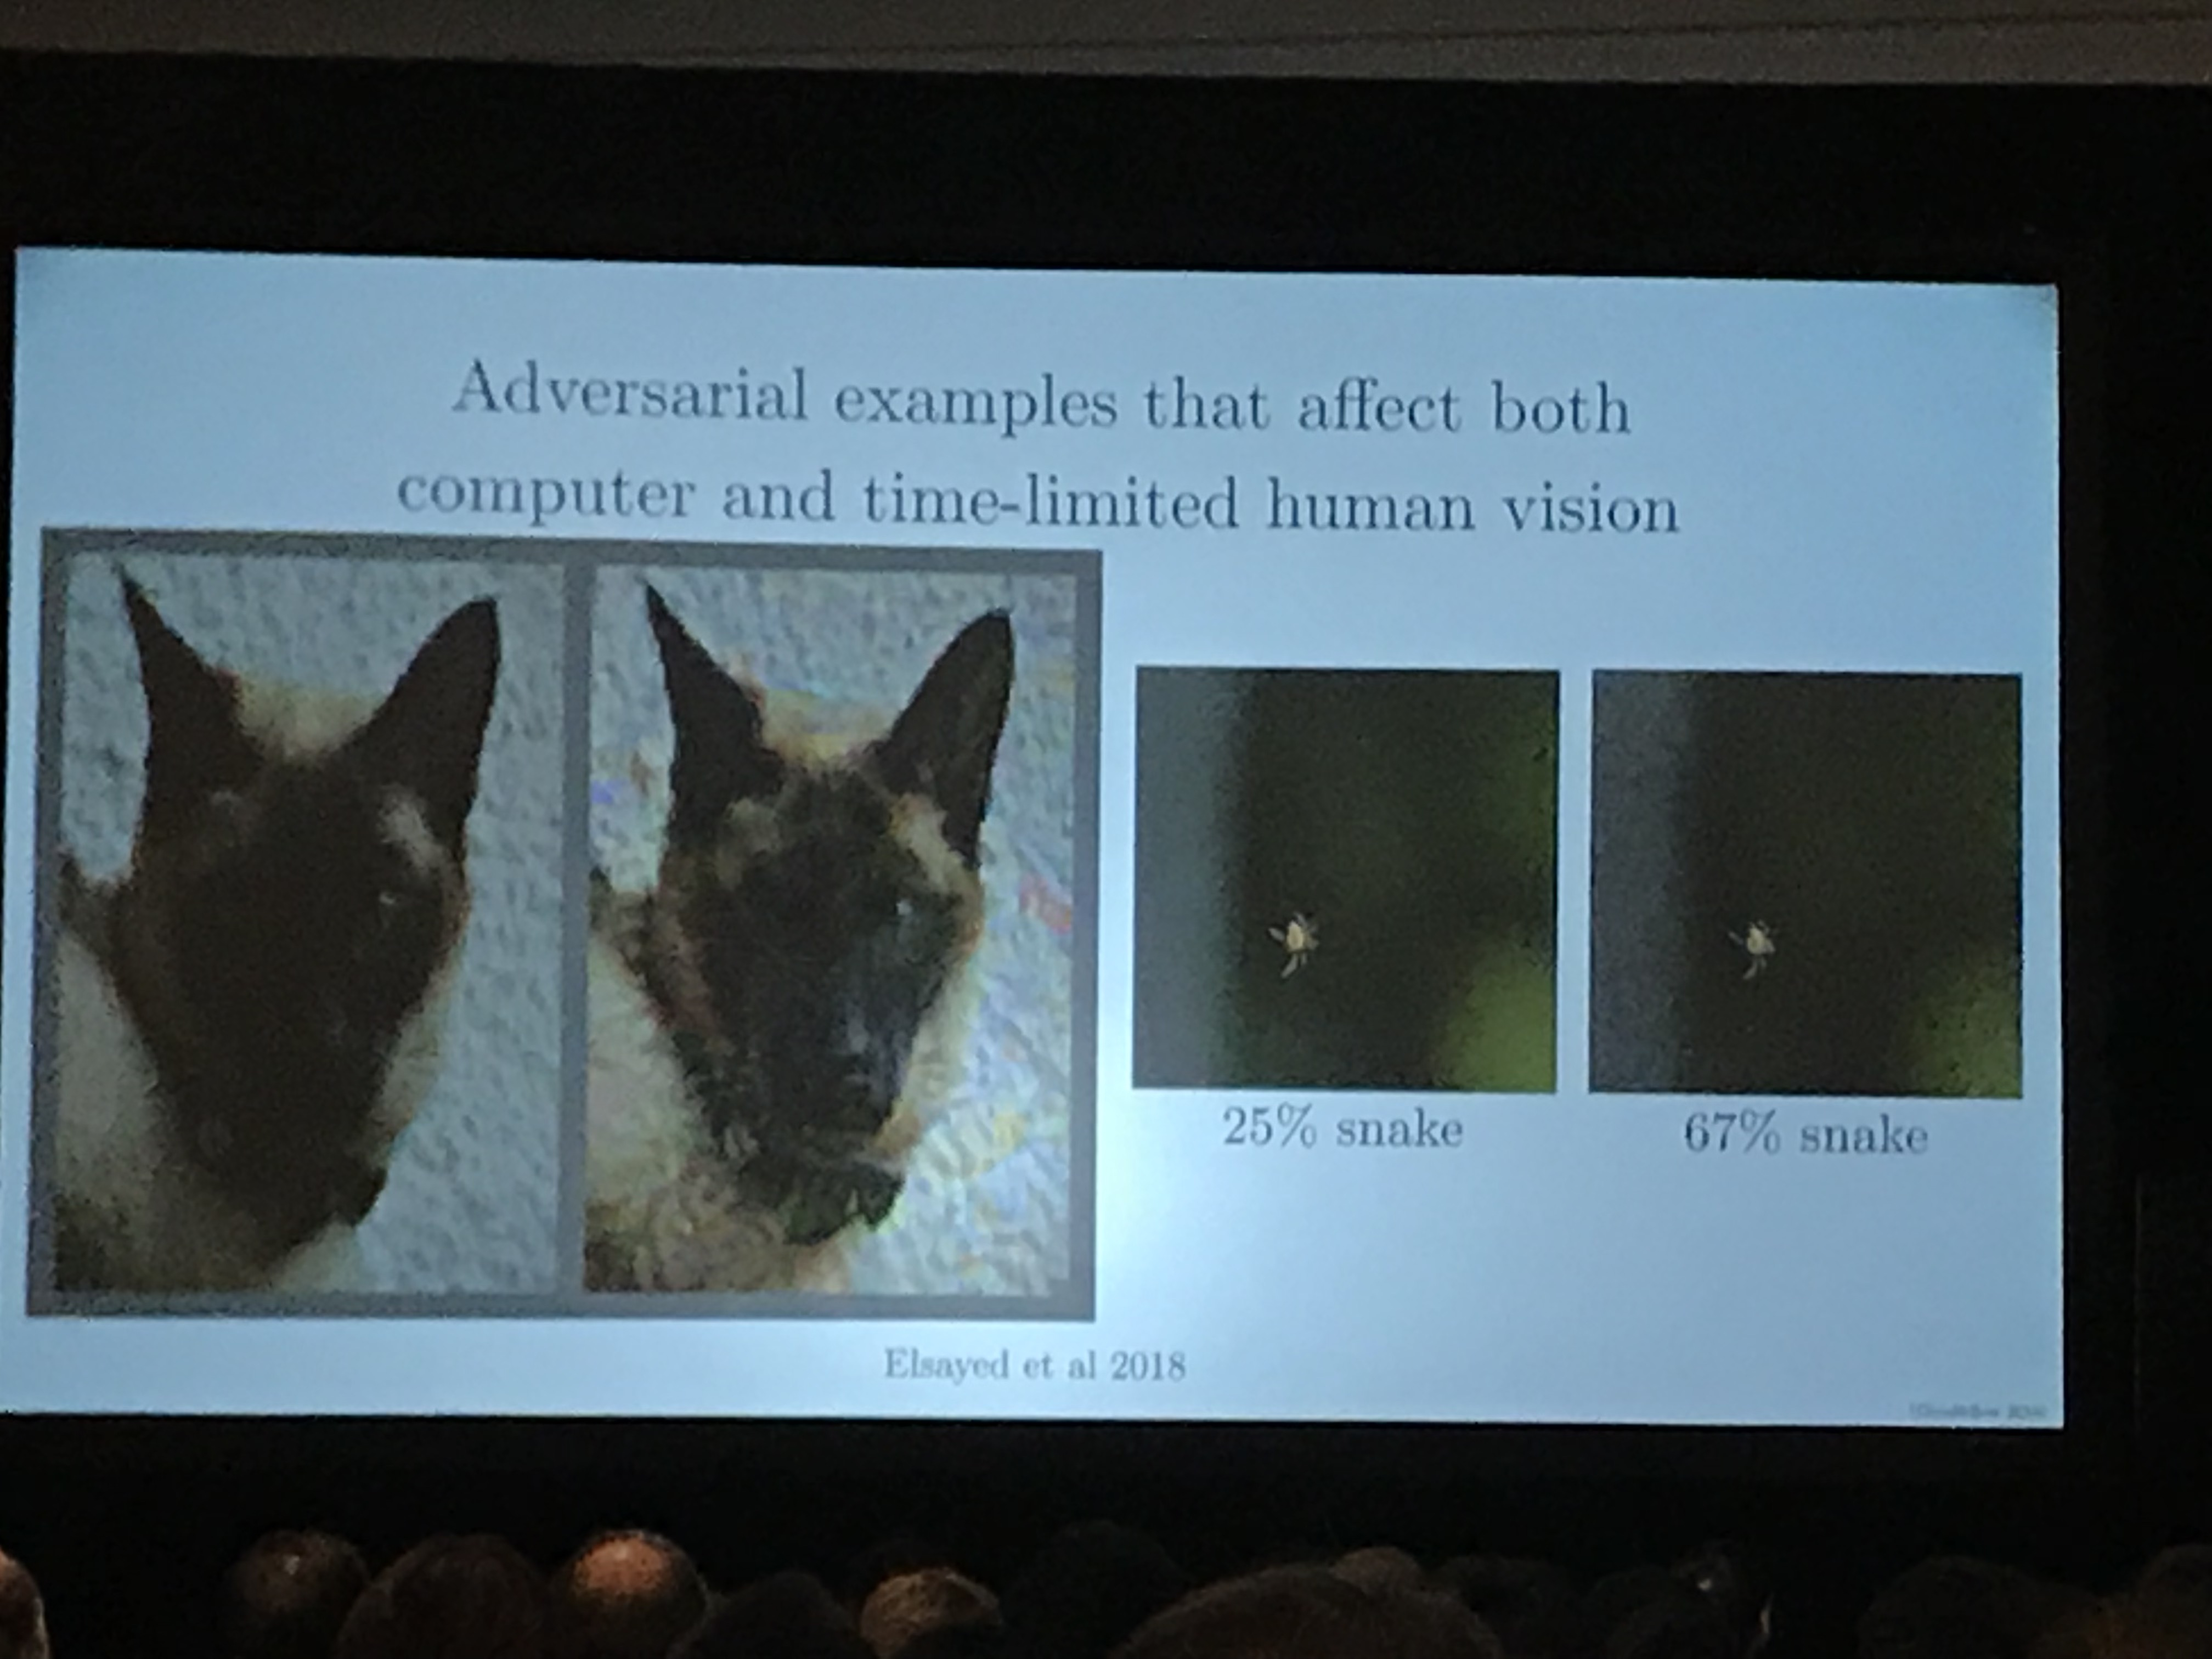
\includegraphics[width=0.5\textwidth]{images/dog.JPG}
    \caption{People are also prone to adversarial examples, too}
    \label{fig:dog}
\end{figure}

\spacerule

\dnote{I have meetings now until the RL session.}

\subsection{Reinforcement Learning}

Now for some RL! (yay!) \\

\subsubsection{Virtual Taobao: Online Environment for RL~\cite{shi2018virtual}}

Paper by Jing-Cheng Shi1, Yang Yu1, Qing Da, Shi-Yong Chen, An-Xiang Zeng. \\

RL is sample inefficient -- so, good virtual environments can be useful. \\

Recommendation in TaoBao is an RL problem. Taobao is an online store like Amazon -- actions involve clicking around, searching, looking at products/reviews, and so on. \\

Claim: RL in TaoBao is infeasible. \\

{\bf Problem:}
\begin{itemize}
    \item User sends search request (can also click/pay/leave).
    
    $\ra$ Goal: optimize customer preference
    
    \item TaoBao displays request (via a ranking policy, $\pi$).
    
    $\ra$ Goal: Maximize performance
\end{itemize}

Main contribution:
\begin{itemize}
    \item Use a GAN-SD (?) to learn a simulated customer policy. Does a good job of simulating the customer's distribution (\dnote{over states? actions? I wasn't sure}).
    \item Then do Multi-Agent Imitation Learning (MAIL) to learn customer shopping policy under a dynamic platform.
    \item Evaluated on TaoBao.
\end{itemize}

\subsubsection{QUOTA: Quantile Option Architecture~\cite{zhang2018quota}}

Distributional RL: Learns a {\it distribution} over the return instead of just the mean. \\

Standard RL: learns $v(s;\theta) \ra \bE[R(\theta)]$. \\

Distributional RL: learns full distribution, $\mc{N}(\mu,\sigma^2)$. \\

{\bf Research Question:} Why need distributional RL?\\

$\ra$ Main answer: can derive risk sensitive policies to explore more effectively. \\

Quantile encoding of a distribution encode {\it rank statistics} of a distribution. Use the median of each quantile to represent that segment. \\

{\bf Quantile-DQN:} Maps each $(s,a)$ to a value distribution of that state-action pair (extension to DQN). \\

Action selection is usually {\it based on the mean} of this distribution. Test on Atari, works better than DQN. Also test on ``roboschool" (similar to mujoco). Also works. \\



Instead: select based on the $k$-th quantile:
\[
a_t = \argmax_a q_k(s,a),
\]
where $k$ is the $k$-th quantile of the value distribution. \\

Bencmarked several algorithms in a simple chain domain to gain intuition -- compare a ``pessimistic"-QR vs. ``optimistic-QR". Can encode optimism/pessimism via choosing high/low quantile. \\

QUOTA: Hierarchical formulation where each quantile is an option.

\subsubsection{Combined RL via Abstract Representations~\cite{franccois2018combined}}

Paper by Vincent Fran{\c{c}}ois-Lavet, Yoshua Bengio, Doina Precup, and Joelle Pineau.\\

{\bf Goal:} Combine model-based and model-free RL to do hierarchical RL. \\

\ddef{Model-basedRL}{learn a model and do planning to compute $Q$.}

\ddef{Model-free RL}{learn $Q$/$\pi$ directly}

Combined! Might be better (more interpretable, sample efficient, and so on). \\

Idea: Combined Reinforcement via Abstract Representations (CRAR). Model-based learns transition function to act, model-free learns value both in an off policy way. \\

Learning: 
$\ra V$, use DDQN.  \\
$\ra T,R$, use an encoder. But! Trivial transition function often learned where all states are abstracted into the same state (which makes $T$ prediction very easy). \\

So, add a regularizer/cost term that encourages more states. \\

Test in a labyrinth task. Yields a meaningful representation that can be visualized in 2dimensions that is interpretable. \\

%Plan based on best estimated $\hat{Q}^*$. \\

Main evaluation on a randomly generated set of labyrinths -- train on a small set of sampled MDPs, then test on a new set of samples. Also do zero-shot transfer on labyrinths. \\

Conclusion:
\begin{itemize}
    \item CRAR can generalize while being efficient
    \item Can work from off policy data
    \item Approach recovers a low-dimensional representation of the environment even in the absence of model-free objective, which is important for 1) transfer, 2) exploration, 3) interpretability.
\end{itemize}

\dnote{Now the poster spotlights, 2 minute highlights}

\subsubsection{Poster Spotlights}

2 minute spotlights:
\begin{itemize}
    \item {\bf Diverse Exploration via Conjugate Policies:} noted that on policy methods suffer from a lack of exploration. Exploration is hard!
    
    $\ra$ solution: diverse exploration. Deploy a set of diverse of exploration policies, where diversity means each policy will behave dissimilarly in each state. 
    
    $\ra$ Contributions: variance analysis of policy gradient objective under these dissimilar exploration policies.
    
    \item {\bf State-Augmentation Transformations:} Look at MDPs in a risk sensitive manner. 
    
    $\ra$ Consider reward functions that take as input $s,a$ {\it and} $s'$. \\
    
    $\ra$ Analzse results if you consider the $(s,a,s')$ based reward function instead of the ``typical" kind. Provide a recipe for translating any transition based MDP to a state based MDP.
    
    \item {\bf Trust Region Evolution Strategies:} Enhance evolution strategies for black box optimization using RL.
    
    $\ra$ Contribution: make more efficient use of sampled data by optimizing surrogate objective function for multiple epochs of updates. Prove guarantees for this next optimization procedure, and a practical algorithm that makes a few approximations.
    
    \item {\bf Comparative Analysis of Expected and Distributional RL:} Where does the advantage of distributuonal RL come from?
    
    $\ra$ Main Q: in what settings does distributional RL behave differently from expected RL?
    
    $\ra$ Conclusions at the poster!
    
    \item {\bf Hybrid RL with Expert State Sequences:} Learning scenario where an RL has access to incomplete but obtainable expert demos.
    
    $\ra$ Propose an efficient dynamics model to infer unobserved actions.
    
    $\ra$ Joint policy optimization via RL and behavioral cloning.
    
    \item {\bf Natural Option Critic:} Builds on Option Critic by combining with Natural Gradients.
    
    $\ra$ Typical Option Critic uses regular gradient which is NOT variant to reparameterization.
    
    $\ra$ Thus, if we extend to natural gradient, we can then do reparameterization, which leads to many practical improvements (without having to invert a matrix).
    
    \item {\bf Utility of Sparse Representations for Control:} Fixed sparse representation like tile coding has been effective for control, but is not scalable b/c number of features explodes.
    
    $\ra$ Goal here is to learn a sparse representation with neural networks (last layer has {\it sparse} activations).
    
    $\ra$ Sparse representation is scalable to high dimensional inputs and is indeed helpful for RL.
    
    
\end{itemize}
